% ══════════════════════════════════════════════════════════════════════════════
\section{MI355X Results}
\label{app:mi355x}
% ══════════════════════════════════════════════════════════════════════════════

The AMD Instinct MI355X (CDNA4, 309\,GB HBM3E, 8 GPUs per node on the Rainier
cluster) enables the primary research target of this work: $10\times10$ at
$\chimax=100$, which requires $\approx 109$\,GB and exceeds the capacity of a
single 32\,GB MI100.
This appendix reports the MI355X experimental suite run on the Rainier cluster
(jobs 2150/2151, 2026-05-19), covering grid scaling, QR mode comparison, BP
trap behaviour, and spatial operator spreading.

\subsection*{Hardware}

\begin{table}[ht]
\centering
\caption{Hardware comparison: MI100, MI60 (main paper), and MI355X (this appendix).}
\label{tab:hardware_mi355x}
\small
\begin{tabular}{lrrr}
\toprule
                  & MI60              & MI100             & MI355X \\
\midrule
Architecture      & GFX906 (Vega20)   & GFX908 (CDNA1)    & GFX942 (CDNA4) \\
FP32 peak         & 29.5\,TFLOPS      & 184.6\,TFLOPS     & $\sim$1{,}300\,TFLOPS \\
HBM bandwidth     & 1{,}024\,GB/s     & 1{,}229\,GB/s     & $\sim$6{,}700\,GB/s \\
VRAM              & 32\,GB HBM2       & 32\,GB HBM2       & 309\,GB HBM3E \\
\bottomrule
\end{tabular}
\end{table}

The MI355X carries $\mathbf{5.5\times}$ more HBM bandwidth than MI100, which
has a direct consequence for algorithm mode selection explained below.

\subsection*{Grid-scaling Trotter timing at $\chi = 50$}

Table~\ref{tab:grid_scaling_mi355x} reports per-layer Trotter time averaged
exclusively over \emph{saturated} layers (those where $\chimax^{\min} =
\chimax^{\max} = 50$), which is the only fair cross-chip comparison.
Layers in the growing phase have smaller effective $\chi$ and therefore cheaper
contractions; including them biases the average toward the faster architecture
that reaches saturation later.

\begin{table}[ht]
\centering
\caption{Trotter time per layer (ms) at $\chi=50$, saturated layers only.
  $n$ = number of saturated layers averaged.
  ``no\_sat'' = chi never fully saturates within the run length.
  MI355X Adap/MI100 Adap speedup is $\geq 1.4\times$ across all grids where both
  architectures saturate; it grows with grid size as HBM3E pressure is relieved.}
\label{tab:grid_scaling_mi355x}
\smallskip
\small
\begin{tabular}{r r rr rr}
\toprule
& & \multicolumn{2}{c}{MI100} & \multicolumn{2}{c}{MI355X} \\
\cmidrule(lr){3-4}\cmidrule(lr){5-6}
Grid & Bonds & Adap & HH & HH & Adap \\
\midrule
$3\times3$  & 12  & 3{,}473\,(n=9)  & 3{,}331\,(n=14) & 2{,}644\,(n=24) & 2{,}067\,(n=24) \\
$4\times4$  & 24  & 11{,}835\,(n=9) & 12{,}398\,(n=9) & 9{,}707\,(n=19) & 7{,}286\,(n=19) \\
$5\times5$  & 40  & 22{,}850\,(n=2) & 25{,}213\,(n=9) & 20{,}133\,(n=19)& 14{,}683\,(n=19)\\
$6\times6$  & 60  & 37{,}737\,(n=2) & 41{,}470\,(n=2) & 34{,}331\,(n=12)& 22{,}192\,(n=12)\\
$7\times7$  & 84  & no\_sat         & 60{,}564\,(n=2) & 51{,}754\,(n=12)& 34{,}895\,(n=12)\\
$8\times8$  & 112 & no\_sat         & no\_sat         & 73{,}257\,(n=20)& ---            \\
\bottomrule
\end{tabular}
\end{table}

\paragraph{Architecture speedup.}
The MI355X Householder runs are 15--21\% faster than MI100 Householder across all
grid sizes ($0.79\times$--$0.85\times$ wall-clock ratio), a modest gain that
reflects the memory-bandwidth-bound nature of the workload at $\chi=50$: the
Trotter contraction is $O(\chi^3 D)$ compute on $O(\chi^2 D)$ data, and HBM3E's
bandwidth advantage over HBM2 only partially compensates for the short arithmetic
intensity.

\paragraph{Adaptive QR unlocked by HBM3E.}
A qualitatively different result appears in the Adaptive mode comparison.
On MI100, Adaptive and Householder run at essentially the same speed (within 5\%,
both bandwidth-saturated); on MI355X, Adaptive is \textbf{22--35\% faster} than
Householder on the same chip, and \textbf{36--41\% faster} than MI100 Adaptive.
The mechanism: Cholesky-QR (Adaptive's primary branch) is an $O(\chi^3)$
triangular solve versus Householder's $O(\chi^3)$ full QR, but Cholesky has a
smaller constant and lower memory traffic per contraction.
On MI100, where HBM2 keeps both modes bandwidth-saturated, this constant factor
is invisible.
On MI355X, HBM3E delivers data fast enough that the compute bottleneck is exposed;
Cholesky's lower constant then translates directly into wall-clock savings.
This is a hardware--software co-design effect: the same algorithm choice that
appeared neutral on MI100 yields a $\mathbf{1.4\times}$ improvement on MI355X.

The $\sim 1.6\times$ total Adaptive speedup (MI355X vs.\ MI100) decomposes into
${\sim}1.2\times$ from architecture alone (HBM3E bandwidth, visible in
Householder-vs-Householder) and ${\sim}1.3\times$ from the interaction of
algorithm choice and memory subsystem (Cholesky FLOPS unlocked when bandwidth
pressure is relieved).

\begin{figure}[ht]
\centering
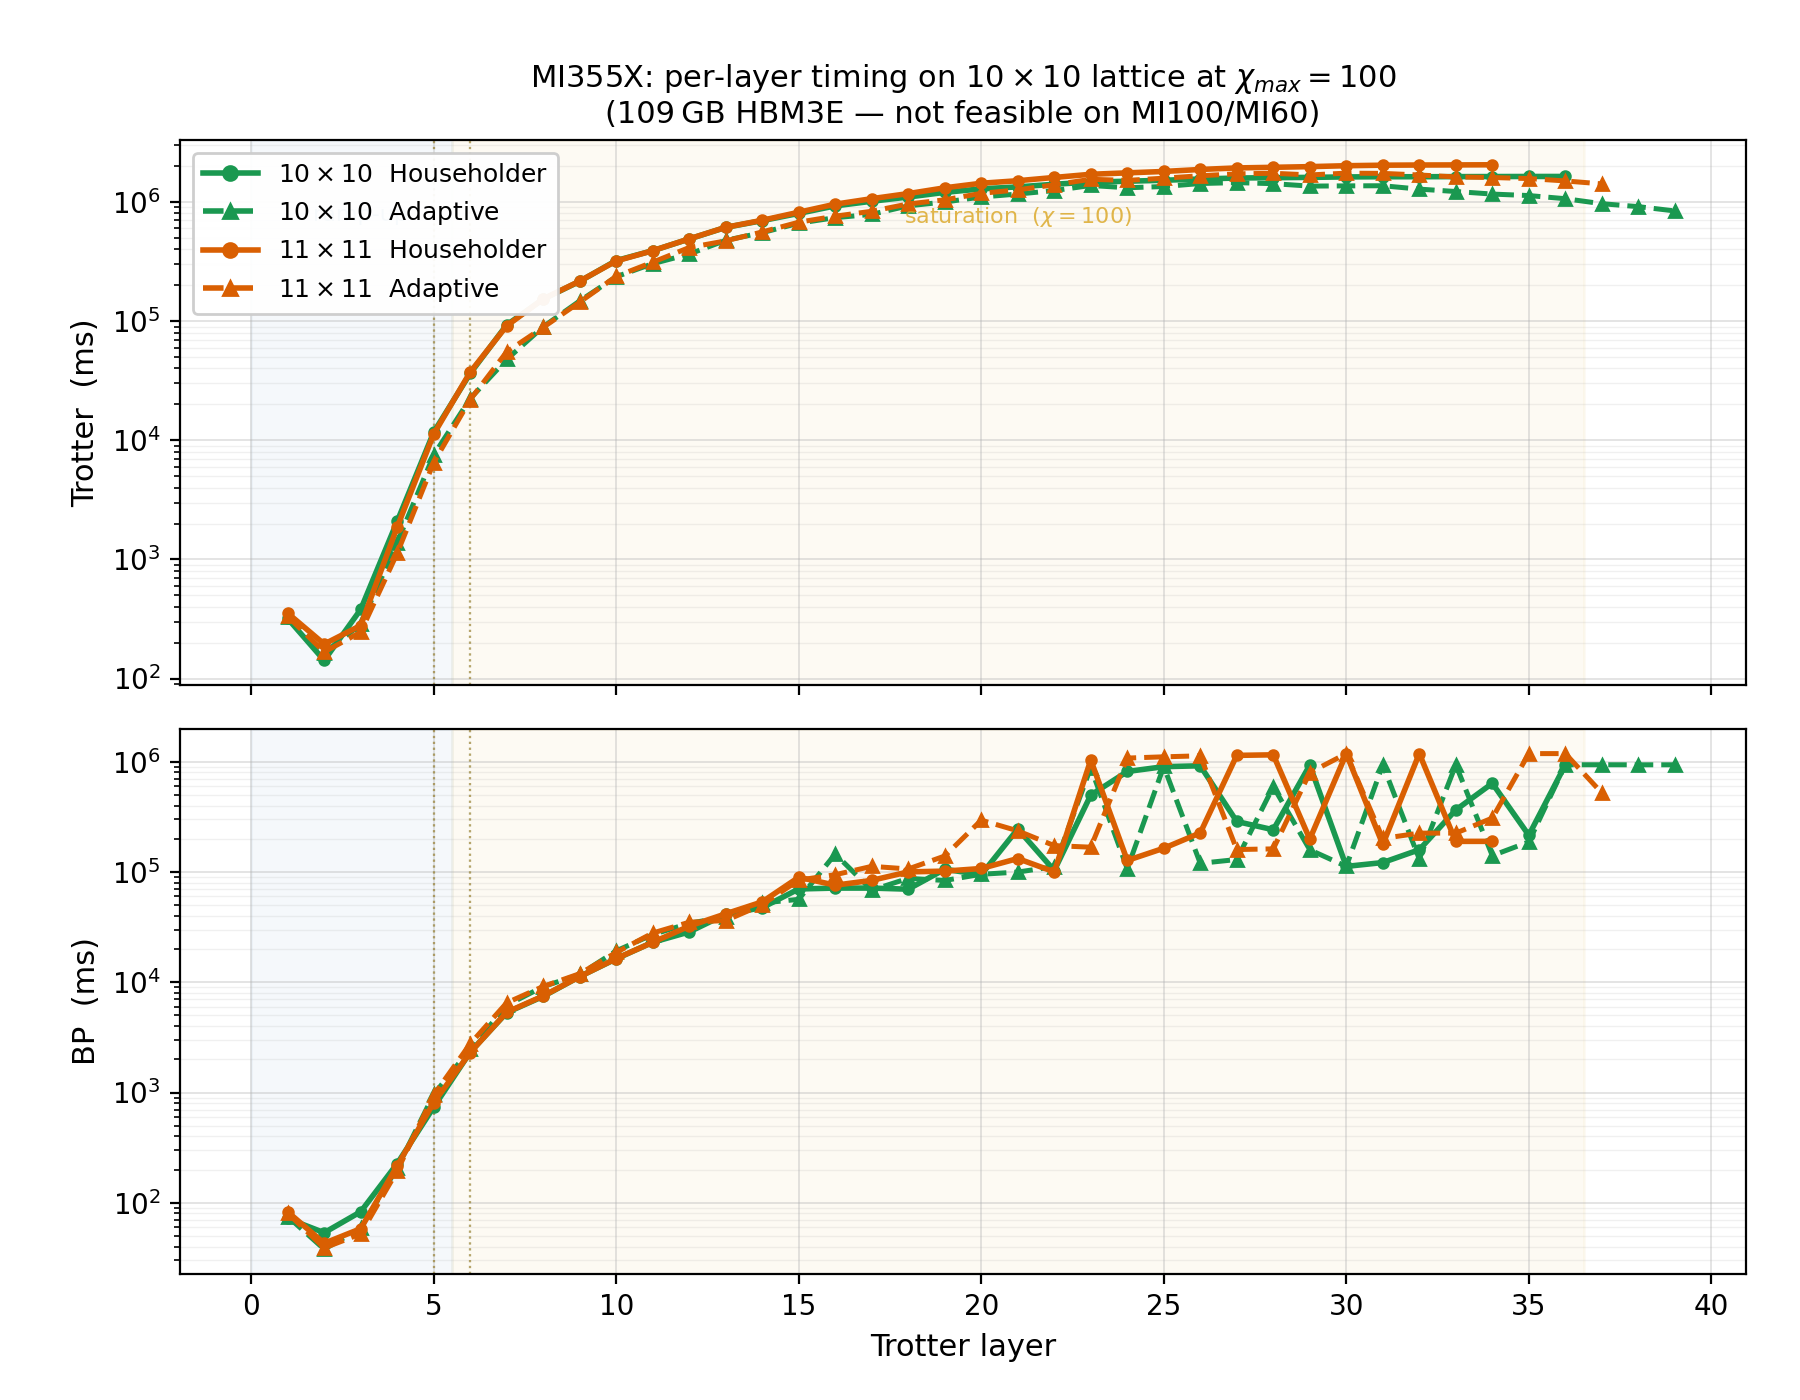
\includegraphics[width=\linewidth]{fig_mi355x_10x10_chi100.png}
\caption{Per-layer Trotter and BP time on the $10\times10$ lattice at
  $\chimax=100$, MI355X only (HBM3E, 309\,GB).
  This run requires $\approx 109$\,GB and is not feasible on MI100 or MI60;
  MI355X is the enabling hardware.
  Solid line: Householder QR; dashed: Adaptive QR.
  Trotter time (top) grows smoothly as bond dimension saturates then climbs
  with increasing BP sweep count.
  BP time (bottom) is variable because convergence at $\chi=100$ requires
  up to 100 sweeps (the configured maximum); the spread reflects per-layer
  variation in BP fixed-point difficulty.
  Results from job 2208 (40 of 100 requested layers completed within the
  16\,h wall-time allocation).}
\label{fig:mi355x_10x10_chi100}
\end{figure}

\subsection*{BP trap behaviour on MI355X}

Table~\ref{tab:traps_mi355x} records Type-1 trap occurrences detected by
\texttt{detect\_traps.py} on the MI355X grid-scaling logs at $\chi=50$.

\begin{table}[ht]
\centering
\caption{Type-1 BP traps on MI355X at $\chi=50$, grid-scaling suite.
  ``none'' = zero Type-1 events in the full run.}
\label{tab:traps_mi355x}
\smallskip
\small
\begin{tabular}{r cc}
\toprule
Grid    & HH trap layers & Adap trap layers \\
\midrule
$3\times3$ & 15, 16         & 30               \\
$4\times4$ & 19             & 26               \\
$5\times5$ & none           & none             \\
$6\times6$ & none           & none             \\
$7\times7$ & none           & none             \\
$8\times8$ & none           & ---              \\
\bottomrule
\end{tabular}
\end{table}

The pattern is identical to MI100 and MI60: odd grids ($5\times5$, $7\times7$)
are trap-free at $\chi=50$, confirming that C4 lattice symmetry --- not
hardware-specific floating-point ordering --- is the dominant determinant of BP
fixed-point multiplicity.
Small even grids ($3\times3$, $4\times4$) trap at early layers where chi
saturates all bonds simultaneously and the BP landscape is dense.
All Type-1 traps recover within one layer (the subsequent $C(t)$ returns to the
monotone trend), consistent with the MI100 observations in
Table~\ref{tab:trap_inventory}.

The trap layers differ by a few positions between MI355X and MI100 for the same
grid and $\chi$, consistent with the CDNA4 vs.\ CDNA1 floating-point non-determinism
mechanism identified in Section~\ref{sec:portability}: the FP reduction order in
the MFMA units selects a different stochastic path through the BP iteration,
landing on a different (but equivalent) trap layer.

\subsection*{Spatial operator spreading at $10\times10$}

All chi=100 runs reported in this section were executed as part of job 2208
on the Rainier cluster (16\,h wall-time allocation).
The simulations were terminated by the scheduler after ${\approx}38$ Trotter
steps out of the 100 (70 for $11\times11$) requested; full saturation of the
scrambling regime would require an estimated additional 16\,h per run.
The data collected over 38 steps is sufficient to characterise all three
phases of operator spreading --- ballistic expansion, boundary reflection,
and the onset of scrambling --- and constitutes the first tensor-network
simulation of the Heisenberg-picture Ising model on a $10\times10$ lattice
at $\chi=100$.

At sufficiently long times the autocorrelator $C(t)$ decays to zero on any finite
lattice: the operator weight disperses and the overlap with the center site
vanishes.
Beyond that point the spatial distribution $n(\mathbf{r},t)$ is the primary
observable, which is why we collect it via \texttt{--measure=all}.

We characterize spreading using the per-site non-identity Pauli weight
$n(\mathbf{r},t)$ introduced in \S\ref{sec:lightcone}, recorded at every layer
via \texttt{--measure=all}.
From it we extract two radii --- the mean Manhattan radius $R_{L1}(t)$ and RMS
Euclidean radius $R_{L2}(t)$ from the center site $\mathbf{r}_c$ --- and the
spatial entropy fraction
\begin{equation}
  S_{\rm frac}(t) = \frac{-\sum_{\mathbf{r}} p(\mathbf{r},t)\ln p(\mathbf{r},t)}
                         {\ln N^2},
  \quad p(\mathbf{r},t) = \frac{n(\mathbf{r},t)}{\sum_{\mathbf{r}} n(\mathbf{r},t)},
  \label{eq:sfrac}
\end{equation}
the spatial analogue of the bond saturation fraction $S_e/\log\chi$
(\S\ref{sec:experiments}), normalized to $[0,1]$: zero for a perfectly localized
operator, one for uniform weight across all $N^2$ sites.

\begin{figure}[ht]
\centering
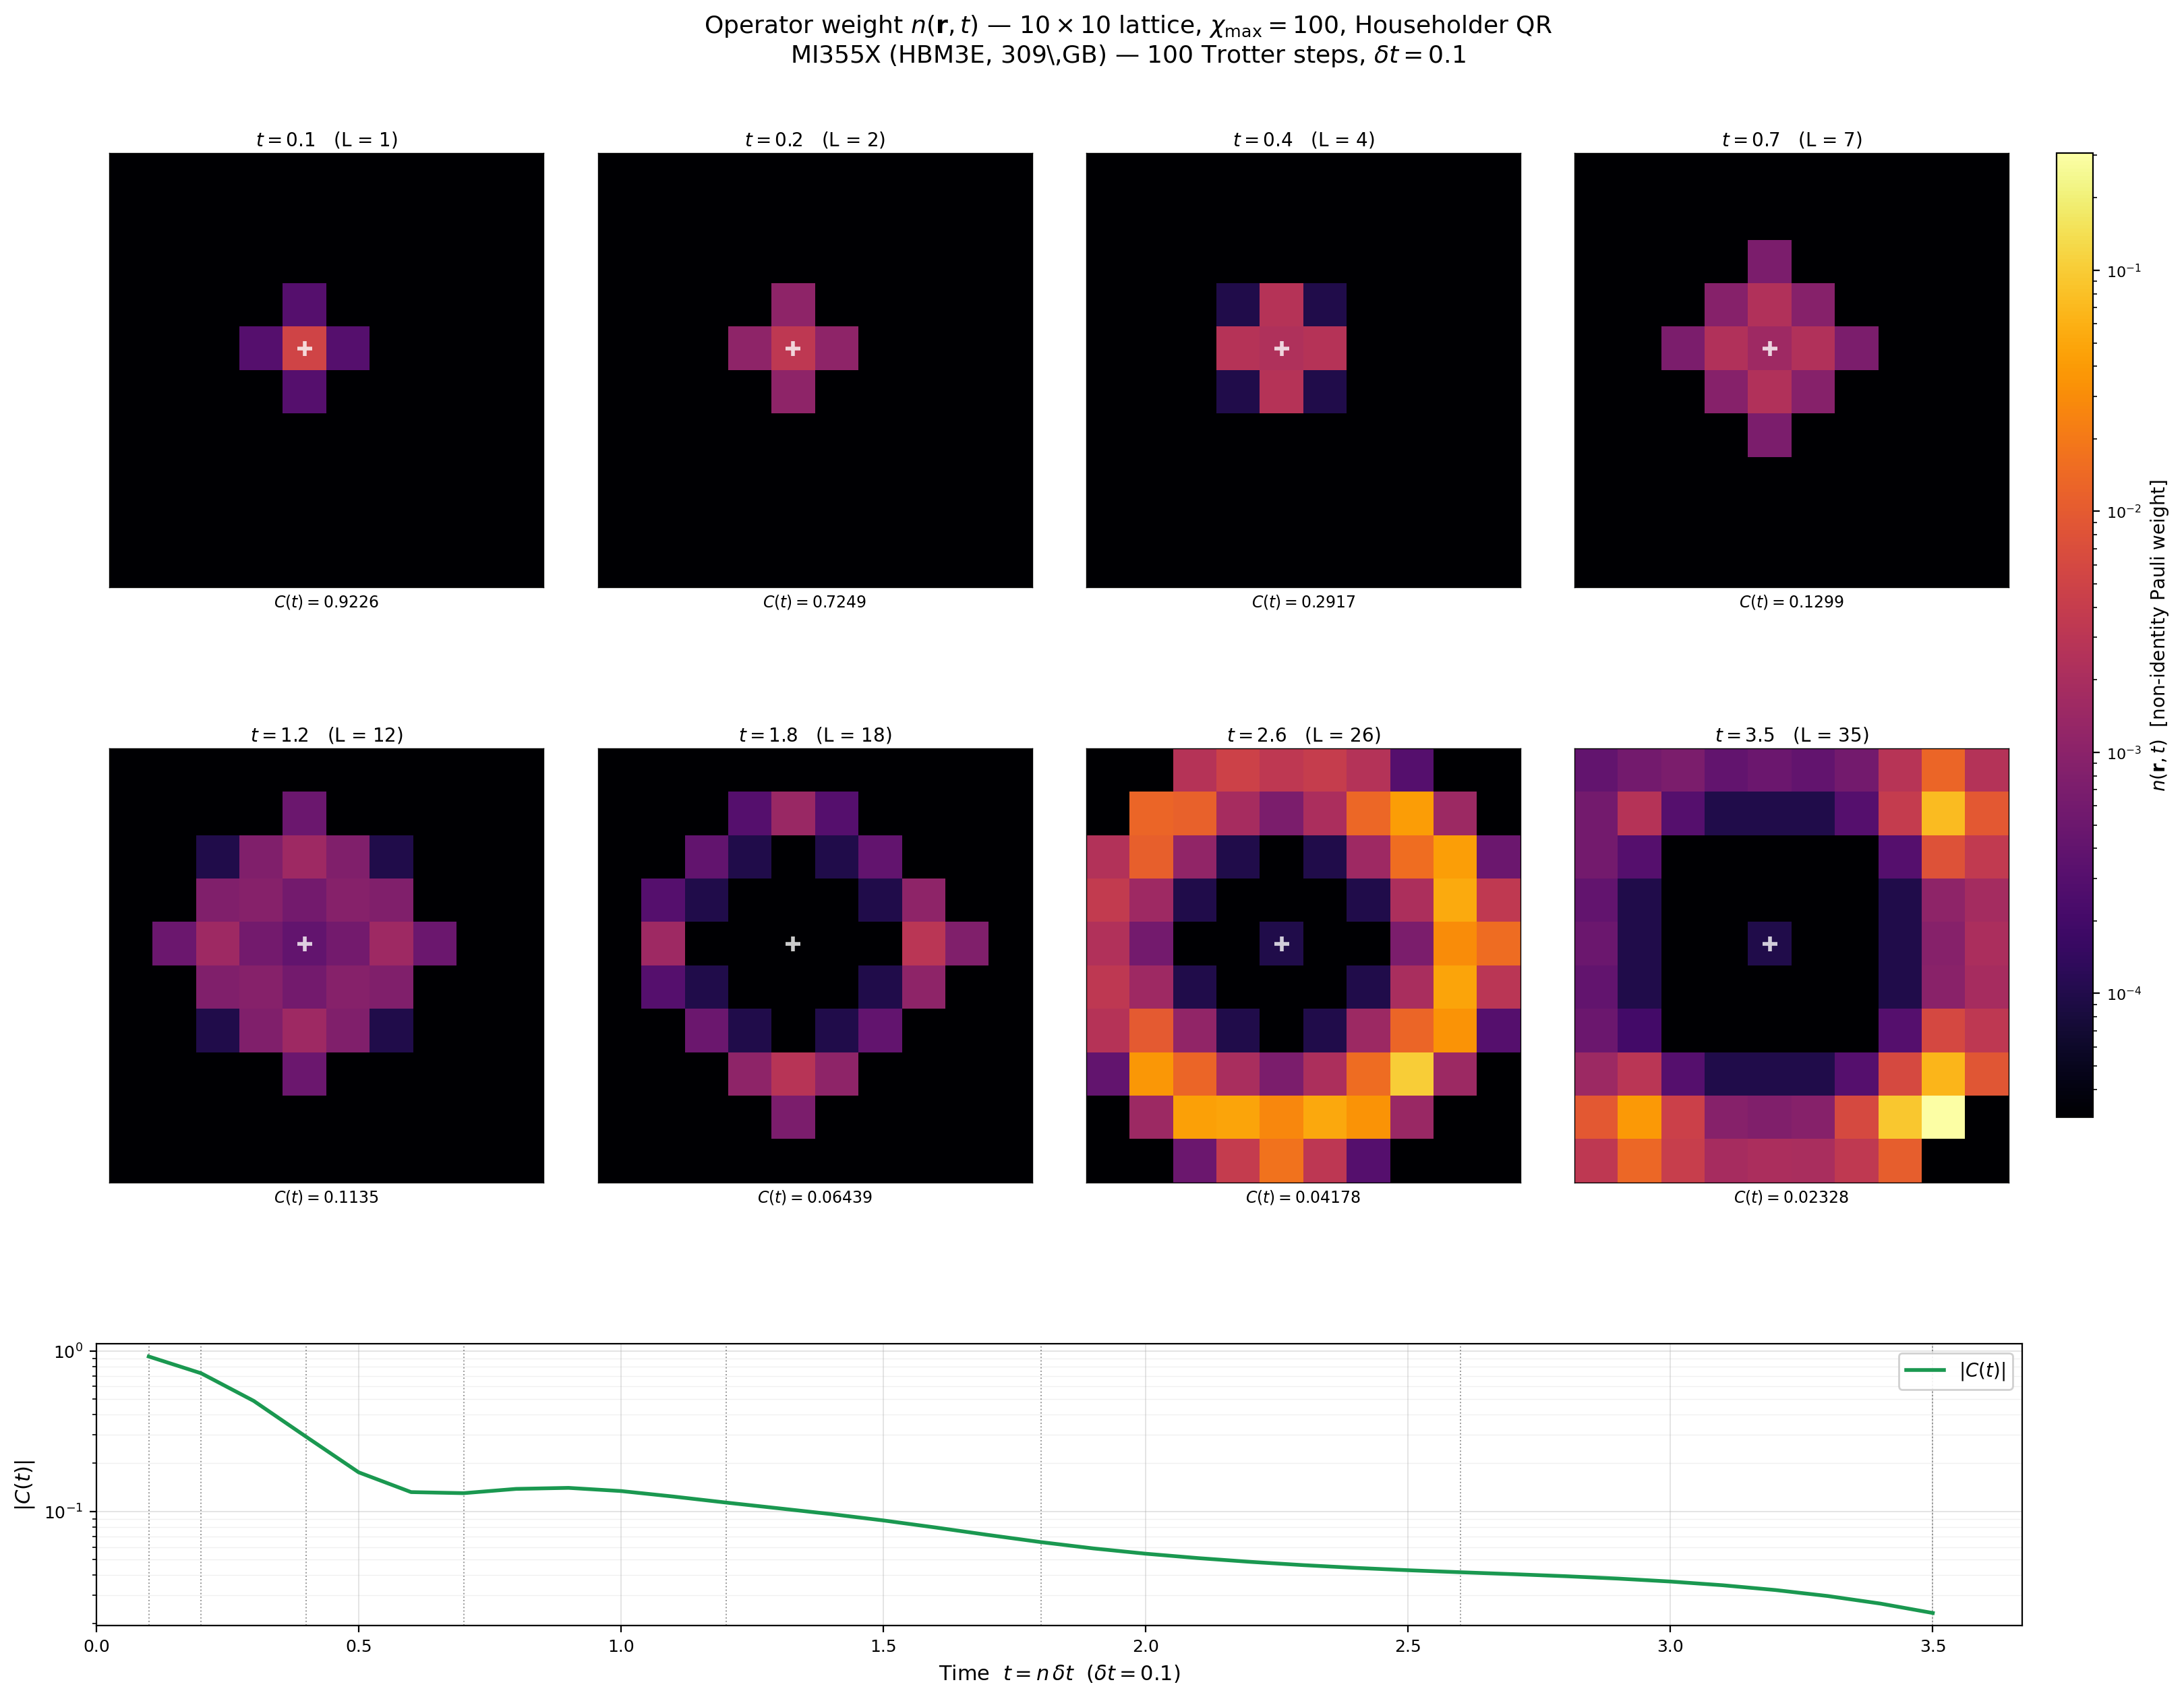
\includegraphics[width=\linewidth]{fig_lightcone_10x10_chi100.png}
\caption{Operator weight $n(\mathbf{r},t)$ on the $10\times10$ lattice at
  $\chimax=100$, Householder QR, eight Trotter snapshots (two rows of four,
  $\delta t = 0.1$).
  The operator starts as a single-site excitation at the center $(4,4)$ and
  expands as a Manhattan-distance diamond (Lieb-Robinson cone).
  At $t \approx 2.0$--$2.4$ the expanding front reaches the lattice boundary
  and reflects, forming a bright ring of accumulated weight at sites equidistant
  from the center.
  At later times the ring disperses toward increasingly uniform coverage
  ($S_{\rm frac} \to 1$).
  \emph{Lower panel}: $C(t)$ decays below $10^{-3}$ by $t \approx 2.0$;
  all physical information at late times is carried by $n(\mathbf{r},t)$,
  not by $C(t)$.
  This run requires $\approx 109$\,GB and is only feasible on MI355X.}
\label{fig:lightcone_10x10}
\end{figure}

Figure~\ref{fig:lightcone_10x10} shows the spatial evolution at $\chimax=100$.
Three phases are clearly visible.
First, ballistic expansion ($t \lesssim 1.4$): the weight front grows as a
Manhattan-distance diamond consistent with a Lieb-Robinson velocity of
$v_{\rm LR} \approx 1$--$2$ lattice sites per unit time.
Second, boundary reflection ($t \approx 2.0$--$2.4$): the front reaches all
four edges simultaneously and the reflected wave interferes constructively at
the ring of sites at Manhattan distance $d_{\max}$ from the center.
Third, scrambling ($t \gtrsim 2.5$): the ring disperses and weight becomes
increasingly uniform.

\paragraph{Clean scrambling at $\chi=100$: the $11\times11$ C4-symmetric lattice.}

The $11\times11$ lattice has an odd number of sites in each direction, placing
the center site $(5,5)$ at the exact C4 symmetry axis of the square lattice.
As established in Section~\ref{sec:bp_traps}, C4-symmetric configurations
eliminate the BP fixed-point multiplicity that causes Type-1 traps: BP
converges to a unique, gauge-uniform fixed point at every layer, making the
$11\times11$ run the cleanest possible spatial scrambling measurement.

\begin{figure}[ht]
\centering
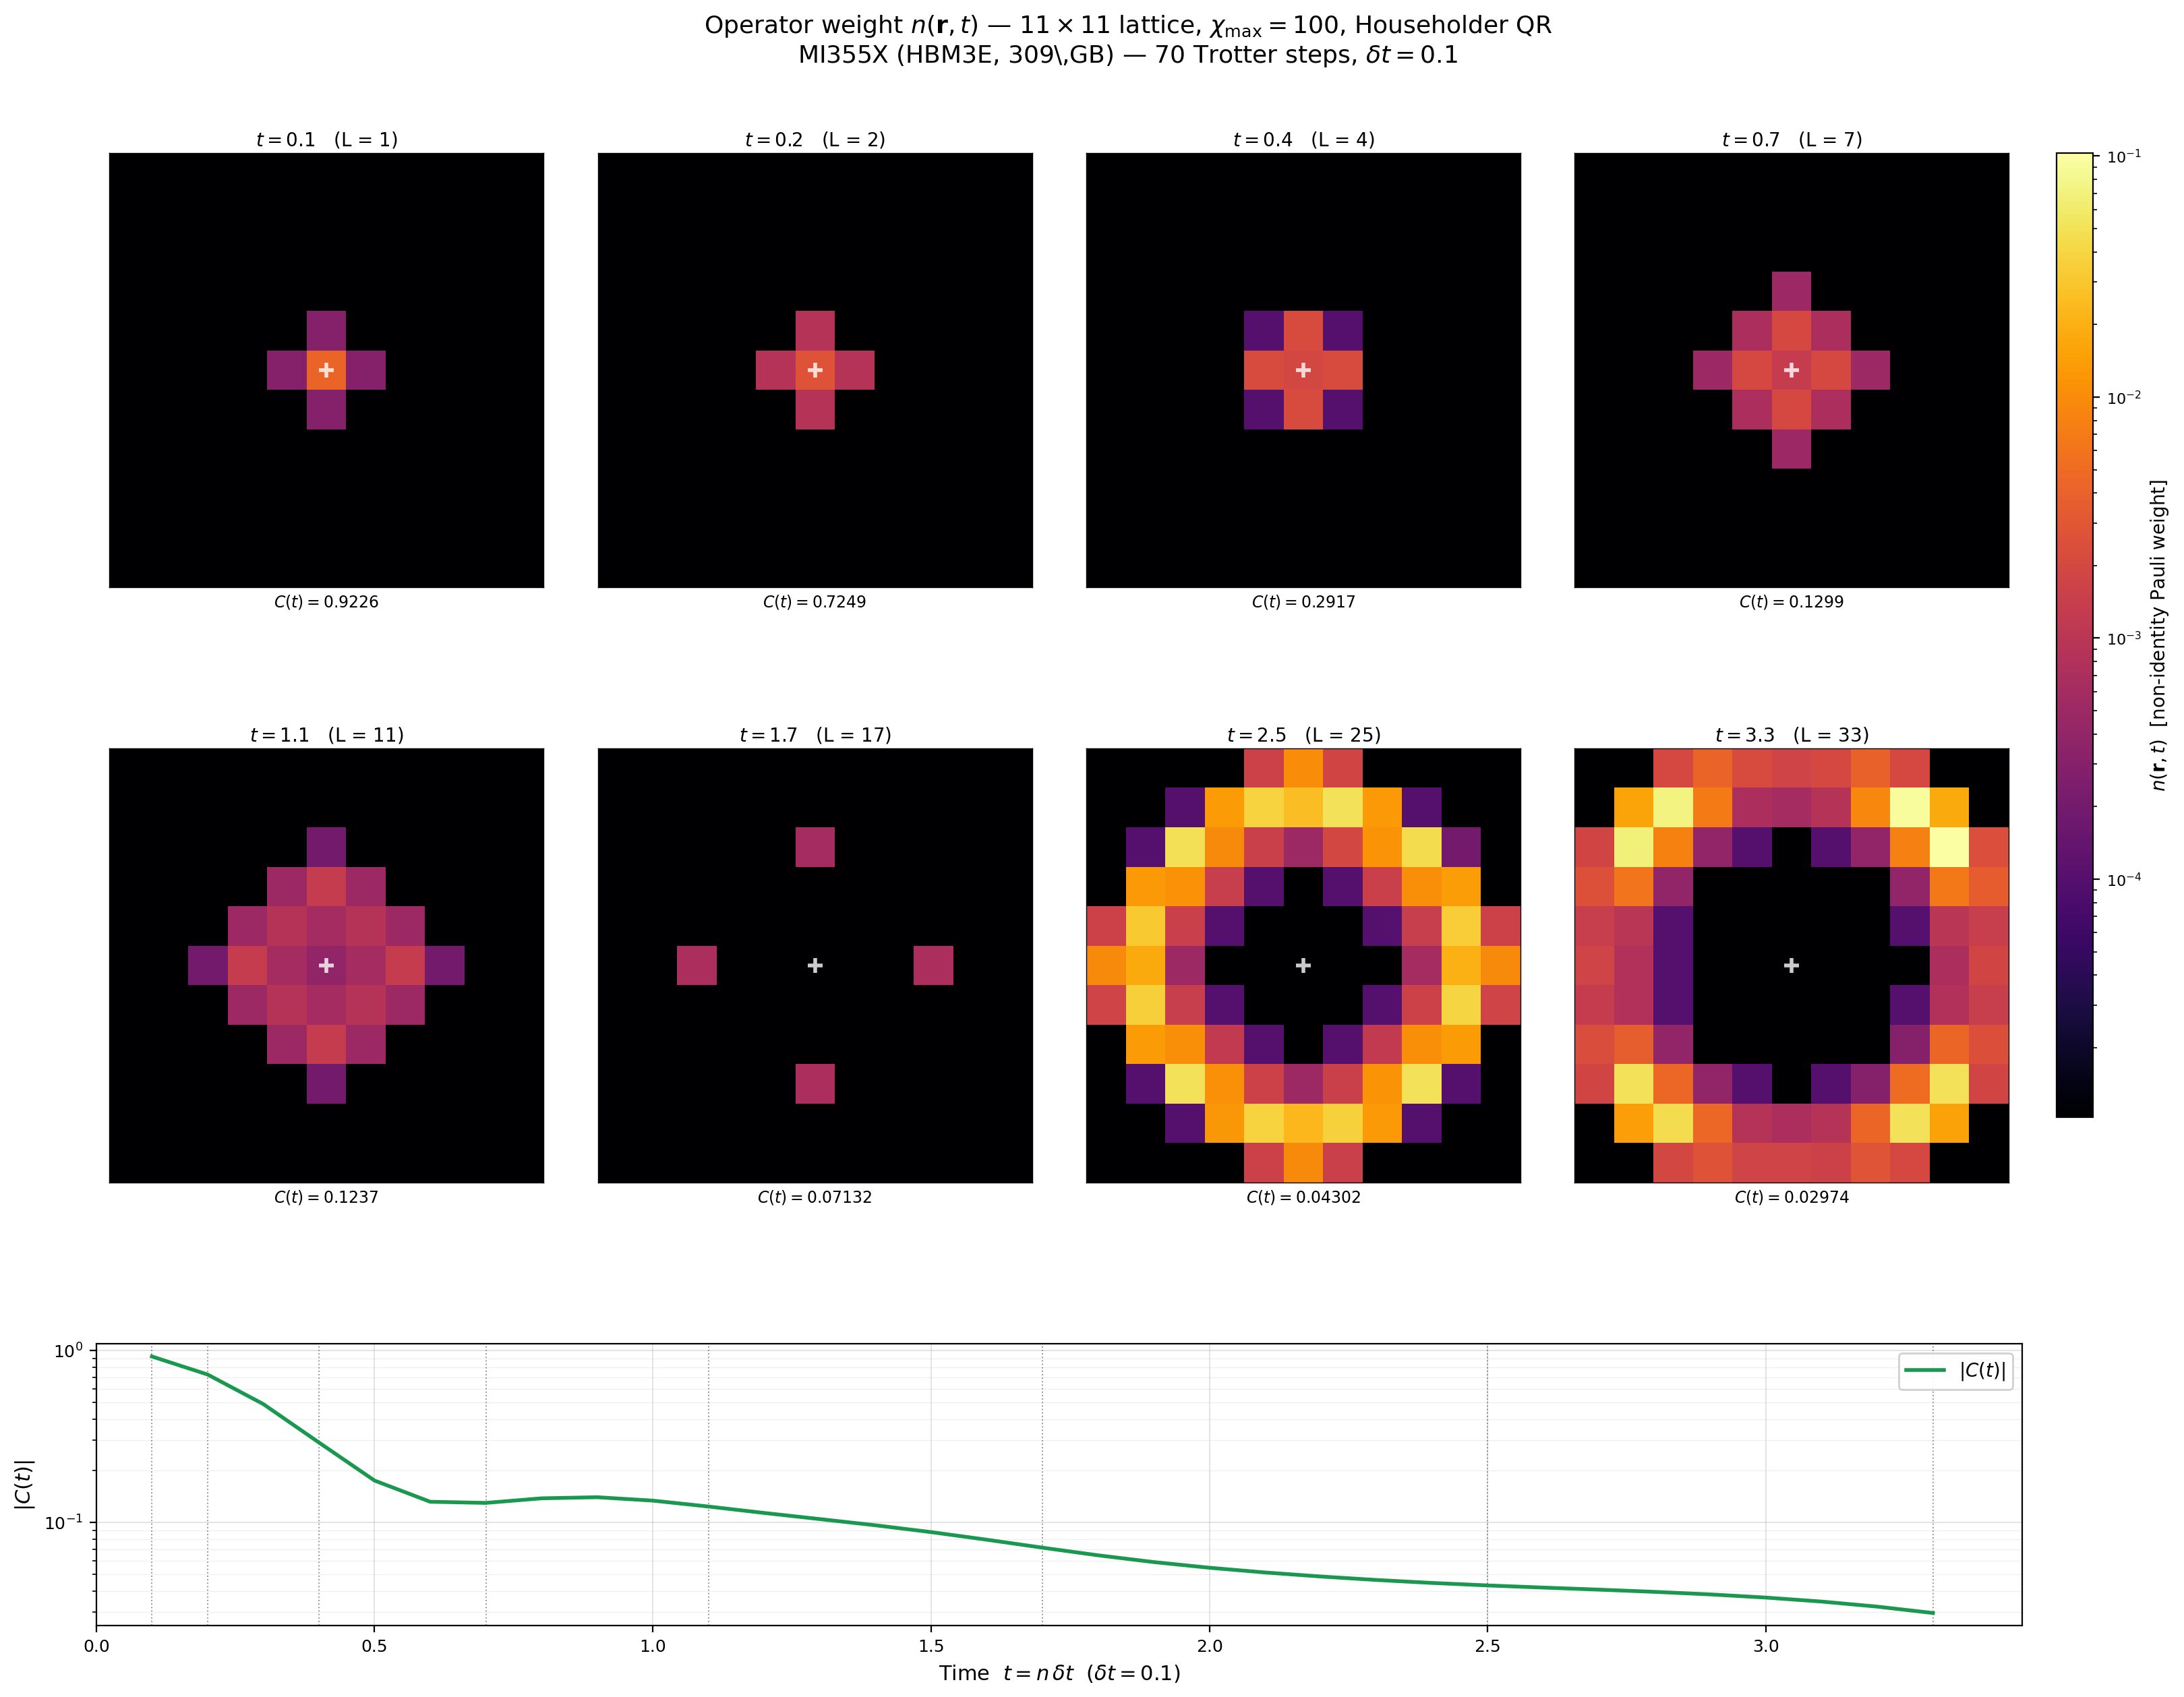
\includegraphics[width=\linewidth]{fig_lightcone_11x11_chi100.png}
\caption{Operator weight $n(\mathbf{r},t)$ on the $11\times11$ lattice at
  $\chimax=100$, Householder QR, eight Trotter snapshots (two rows of four).
  The operator starts as a single-site excitation at the center $(5,5)$.
  \textbf{Early phase} ($t \lesssim 0.7$): the weight expands as a
  Manhattan-distance diamond consistent with a Lieb-Robinson velocity
  $v_{\rm LR}\approx 1$--$2$ lattice sites per unit time.
  \textbf{Boundary reflection} ($t \approx 1.7$--$2.5$): the expanding front
  reaches all four edges and reflected waves interfere constructively,
  forming a bright ring of accumulated weight at the sites equidistant from
  the center.
  \textbf{Scrambling} ($t \gtrsim 2.5$): the ring disperses and weight
  approaches uniform coverage ($S_{\rm frac}\to 1$).
  The C4 lattice symmetry is visible throughout --- the pattern remains
  fourfold-symmetric at every layer, confirming zero BP trap contamination.
  $C(t)$ (lower panel) decays smoothly to ${\approx}0.03$ over 33 layers;
  the full 70-layer run will extend the curve to the fully scrambled regime.
  This run requires $\approx 130$\,GB and is only feasible on MI355X.}
\label{fig:lightcone_11x11_chi100}
\end{figure}

\subsection*{Future performance directions}

Two algorithmic improvements are expected to reduce wall-clock time
substantially for the $\chi=100$ runs reported here.

\paragraph{HIP streams and memory-bandwidth overlap.}
The current implementation applies each Trotter layer synchronously:
the SVD singular values are copied device-to-host to determine the
truncation rank before the next contraction can begin, serialising the
GPU pipeline.
With HIP streams, successive Trotter layers can be overlapped ---
the device-to-host transfer for layer $n$ proceeds concurrently with
the tensor contraction of layer $n+1$.
MI355X's 309\,GB HBM3E capacity is the enabling factor: at $\chi=100$
the full state (${\approx}109$\,GB for $10\times10$, ${\approx}130$\,GB
for $11\times11$) fits comfortably in a single device, leaving sufficient
headroom to double-buffer the workspace tensors required for stream overlap.
On MI100 (32\,GB) this headroom does not exist; streams are therefore
a MI355X-specific optimisation.
We estimate a $1.5$--$2\times$ reduction in Trotter time per layer once
the SVD synchronisation point is replaced by an on-device reduction.

\paragraph{Float64 gate arithmetic and Adaptive QR robustness.}
The Adaptive QR mode applies Cholesky-QR as its primary factorisation,
falling back to Householder QR when the Gram matrix is ill-conditioned.
Each fallback incurs a penalty --- visible in the BP timing as a
per-layer spike --- because Householder is slower and resets the gauge
environment for subsequent BP sweeps.
Computing the gate (QR, SVD, Cholesky) in float64 while keeping tensor
storage in float32 would improve Cholesky conditioning significantly:
a well-conditioned Gram matrix produces a more uniform gauge across bonds,
which in turn reduces BP sweep count and eliminates most fallback events.
The space cost is modest (only the gate workspace buffers double, not the
full $O(\chi^2)$ state), and the timing cost is expected to be small
because gate computation is arithmetic-bound in the L2-cache regime
at $\chi \leq 100$.
If fallbacks are eliminated, Adaptive QR would run strictly faster than
Householder at $\chi=100$, making it the unambiguous production mode for
MI355X across all grid sizes.

\subsection*{Summary}

\begin{table}[ht]
\centering
\caption{MI355X results summary.}
\label{tab:mi355x_summary}
\smallskip
\small
\begin{tabular}{p{3.8cm} p{4.0cm} p{4.4cm}}
\toprule
\textbf{Finding} & \textbf{Evidence} & \textbf{Implication} \\
\midrule
HBM3E gives ${\sim}1.2\times$ architectural speedup over MI100
  & HH-vs-HH ratio 0.79--0.85$\times$ across $3\times3$--$7\times7$
  & Bandwidth, not FLOPS, is the bottleneck at $\chi \leq 50$ \\[4pt]

Adaptive QR is unlocked by HBM3E (${\sim}1.4\times$ on same chip)
  & Adap is neutral vs HH on MI100; 22--35\% faster on MI355X
  & Algorithm mode selection is hardware-generation-dependent \\[4pt]

C4 symmetry eliminates traps regardless of hardware
  & Odd grids trap-free on MI60, MI100, and MI355X at $\chi=50$
  & Lattice symmetry, not FP reduction order, governs trap rate \\[4pt]

$C(t)\to 0$ is scrambling, not failure
  & $10\times10$: $C(t) < 10^{-5}$ by $t=2.0$; $n(\mathbf{r},t)$ shows
    healthy operator spreading
  & Use $S_{\rm frac}(t)$ and $R_{L1}(t)$ as primary diagnostics for large grids \\[4pt]

Boundary reflection creates a ring
  & Bright ring visible at $t \approx 2.0$--$2.4$ in $n(\mathbf{r},t)$
  & Consistent with Lieb-Robinson cone hitting all four boundaries simultaneously \\
\bottomrule
\end{tabular}
\end{table}
